Once you have activated \bxpref{TeststyleActivate} and configured \bxpref{TeststyleConfigure} Teststyle for a \gdproject{}, you will be informed when your chosen guidelines are not being upheld. The central place for viewing your Teststyle information, warnings and errors is the \gdprobview{}.

For each Teststyle message, you will see an entry in the \gdprobview{}, with the information on where the guideline is not being upheld. You can use the \gdprobview{} to view the rule that has been flouted and also to fix the problem using the Quick Fix option. 

\subsubsection{Viewing the broken Teststyle rule from the \gdprobview{}}
\begin{enumerate}
\item Select the entry in the \gdprobview{} whose rule you want to view.
\item Right-click in the \gdprobview{} and select:\\
\bxmenu{Show Teststyle Rule}{}{}\\
from the context-sensitive menu.
\item The \gdproject{} properties dialog appears, opened at the Teststyle page. The guideline that resulted in the entry in the \gdprobview{} is selected. 
\item From here you can adapt the guideline if required \bxpref{TeststyleConfigure}. 
\end{enumerate}

\subsubsection{Using Quick Fix to fix the problem}

\begin{enumerate}
\item Select the entry or entries you want to work on from the \gdprobview{}.
\item Right-click in the \gdprobview{} and select:\\
\bxmenu{Quick Fix}{}{}\\
from the context-sensitive menu.
\item The Quick Fix dialog \bxfigref{quickfix} will appear with the options available to fix the problem. The options may range from opening an editor to automatically fixing the problem.
\item Select the option(s) you want to carry out and click \bxcaption{OK}.
\item The option(s) you chose will be executed. 
\end{enumerate}

\begin{figure}[p]
\begin{center}
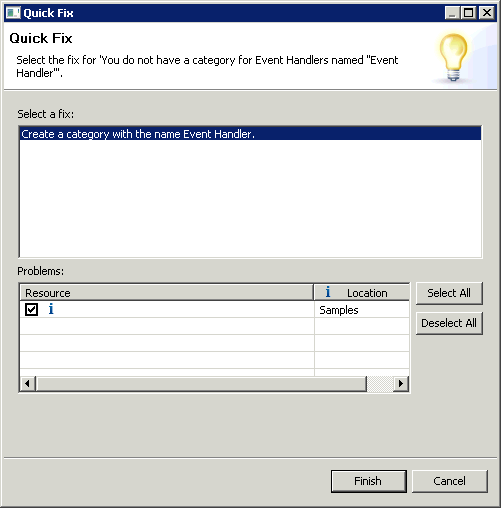
\includegraphics{Tasks/Teststyle/PS/quickfix}
\caption{Quick Fix}
\label{quickfix}
\end{center}
\end{figure}
